%!TEX root = ../thesis.tex
%*******************************************************************************
%****************************** Third Chapter *********************************
%*******************************************************************************

\chapter{Mean level eQTL mapping using single cell RNA-seq data from iPSCs}

Traditional eQTL mapping uses, as a measure of gene expression, bulk RNA-sequencing, where expression level is averaged out across all cells from a given individual (section 1.1).
Recent advances in experimental techniques allow to assess gene expression at the single cell level.
The first single-cell RNA sequencing (scRNA-seq) experiment was published in 2009, and the authors profiled only eight cells \cite{tang2009mrna}. 
Only 7 years later, 10X Genomics released a data set of more than 1.3 million cells (ref).
Today, over 1,000 scRNAseq datasets have been published (ref).
By now scRNAseq is an established technique and methods are available to efficiently and reliably perform both low level and complex tasks such as clustering and pseudotime estimation (refs).\\

With the ability to identify cell types and states in an unbiased manner the use of scRNA-seq data is uniquely positioned to provide an extra layer to our understanding of genetic regulation of expression across a plethora of cell types and states.
As a consequence, single cell eQTL mapping (where scRNAseq profiles are combined with genotype information) is slowly emerging as a field and it promises to greatly help our understanding of the architecture of human disease across tissues \cite{van2018single, cuomo2020single, jerber2020population, van2020single}.
As more and more studies emerge, it becomes important to establish a "best practice" pipeline to optimise yield of sc eQTL studies and uniform methods across the field.\\

Here, we leverage matched bulk and single cell gene expression of human iPSCs lines from around 100 donors to identify general guidelines for eQTL mapping using scRNAseq data.
We compare several manners of normalising and aggregating expression across cells per donor as well as different models to test for eQTL and compare to equivalent results obtained when using bulk RNA seq data.
Whilst for most individuals we have plate-based scRNAseq data (SmartSeq2, \cite{picelli2013smart}), we also have data using the 10X Genomics platform \cite{} for a subset of around 30 samples, which allows us to an extent to also compare results across single cell technologies.

\begin{Abstract}
% \subsection{Contributions}
\hspace{-3mm}\textbf{Contributions} This work was done in collaboration between the Stegle and McCarthy labs and was published in \cite{}.\\

The code for processing, analysing and plotting the data is open source and freely accessible here:

The paper was written in collaboration with Giordano Alvari and Marc Jan Bonder, and is available at .
\vfill
\end{Abstract}

\section{What is different in single cell data?}

When we perform eQTL mapping, we are interested to find differences in expression level between individuals, as a function of their different genotypes as specific genomic loci. 
Under the assumption that we are looking at an otherwise homogeneous population of cells (e.g. all cells of a given cell type) it is reasonable to take the sum or the average expression per individual, across all cells.
When we use bulk RNA sequencing expression profiles, that is essentially what happens: all cells from an individual are pooled, the mRNA extracted and sequenced. 
The resulting reads are and mapped onto a reference genome, and the expression level of each gene is quantified as the number of reads obtained from one donor that uniquely map to that gene. 
A bulk RNA-seq experiment, therefore, results in one individual measure of “abundance” of each gene for each donor. 
Such measure is the results of aggregating over XX cells [REF] and, at least for expressed genes (average TPM > YY) follows a distribution that can be approximated as Gaussian.\\

The intuition here is that 
% Pool of RNA transcripts from many genes (low probability for a given gene), get a sample to sequence. 
% Poisson: sampling from large n, small p (samples are technical replicates)
% (biological replicates - NB > Poisson, larger variance )

% As discussed in section 1.3 of the Introduction, 
Recent advances in experimental technologies have provided robust methods for single-cell RNA sequencing (scRNA-seq), allowing to assay the genome-wide transcriptome of hundreds to thousands of individual cells. 
Whilst scRNA-seq data provides increased resolution and promises great insights into our understanding of cellular function, the data also is much sparser, and the amount of cells that can be assayed for an individual is limited compared to bulk (add numbers).
In general, we observe a smaller number of cells and therefore total reads for an individual as compared to bulk. 
In addition, the read distribution is far from Gaussian, with very different amount of reads coming from different donors. 
This is in part due to the "double sampling" that is inherent of the technology: there is a chance of not sampling any reads from one gene in one cell, and there is a chance of not sequencing any reads from that cell at all.

% Add differences in number of total reads, read distribution, describe “double sampling” process.

\section{Methods}

In order to produce bulk-like results, two main approaches can be used.

Under the assumption that we are looking at a single cell type, we can i) aggregate counts across all cells from an individual (e.g. taking the average expression value) and generate a "pseudo-bulk" measure, and then run the test exactly as if it were bulk; or ii) use full single cell expression, without aggregating.

% In this chapter, we introduce the two datasets that we will use throughout the thesis, setting the scene for all other chapters. 
% These are among the very first datasets of their kind, assessing single cell gene expression profiles for hundreds of genetically diverse individuals, allowing to interrogate the effect of common genetic variation on transcriptional variability.
% Previously, most eQTL mapping studies in humans were performed using bulk RNA-sequencing, and most scRNA-seq studies were performed in a handful of individuals only, or in model organisms (often also limited to a few strains).
% Notably, one study performed eQTL mapping using scRNA-seq \cite{van2018single} recently in blood cells. 
% However, this data is limited to 45 individuals and to a single time point, lacking the differentiation axis of our studies.

\subsection{Datasets}

\begin{itemize}
    \item iPS data
    \item simulated data
\end{itemize}

\subsection{Aggregation strategies}

% add workflow figure

\begin{figure}[h]
\centering
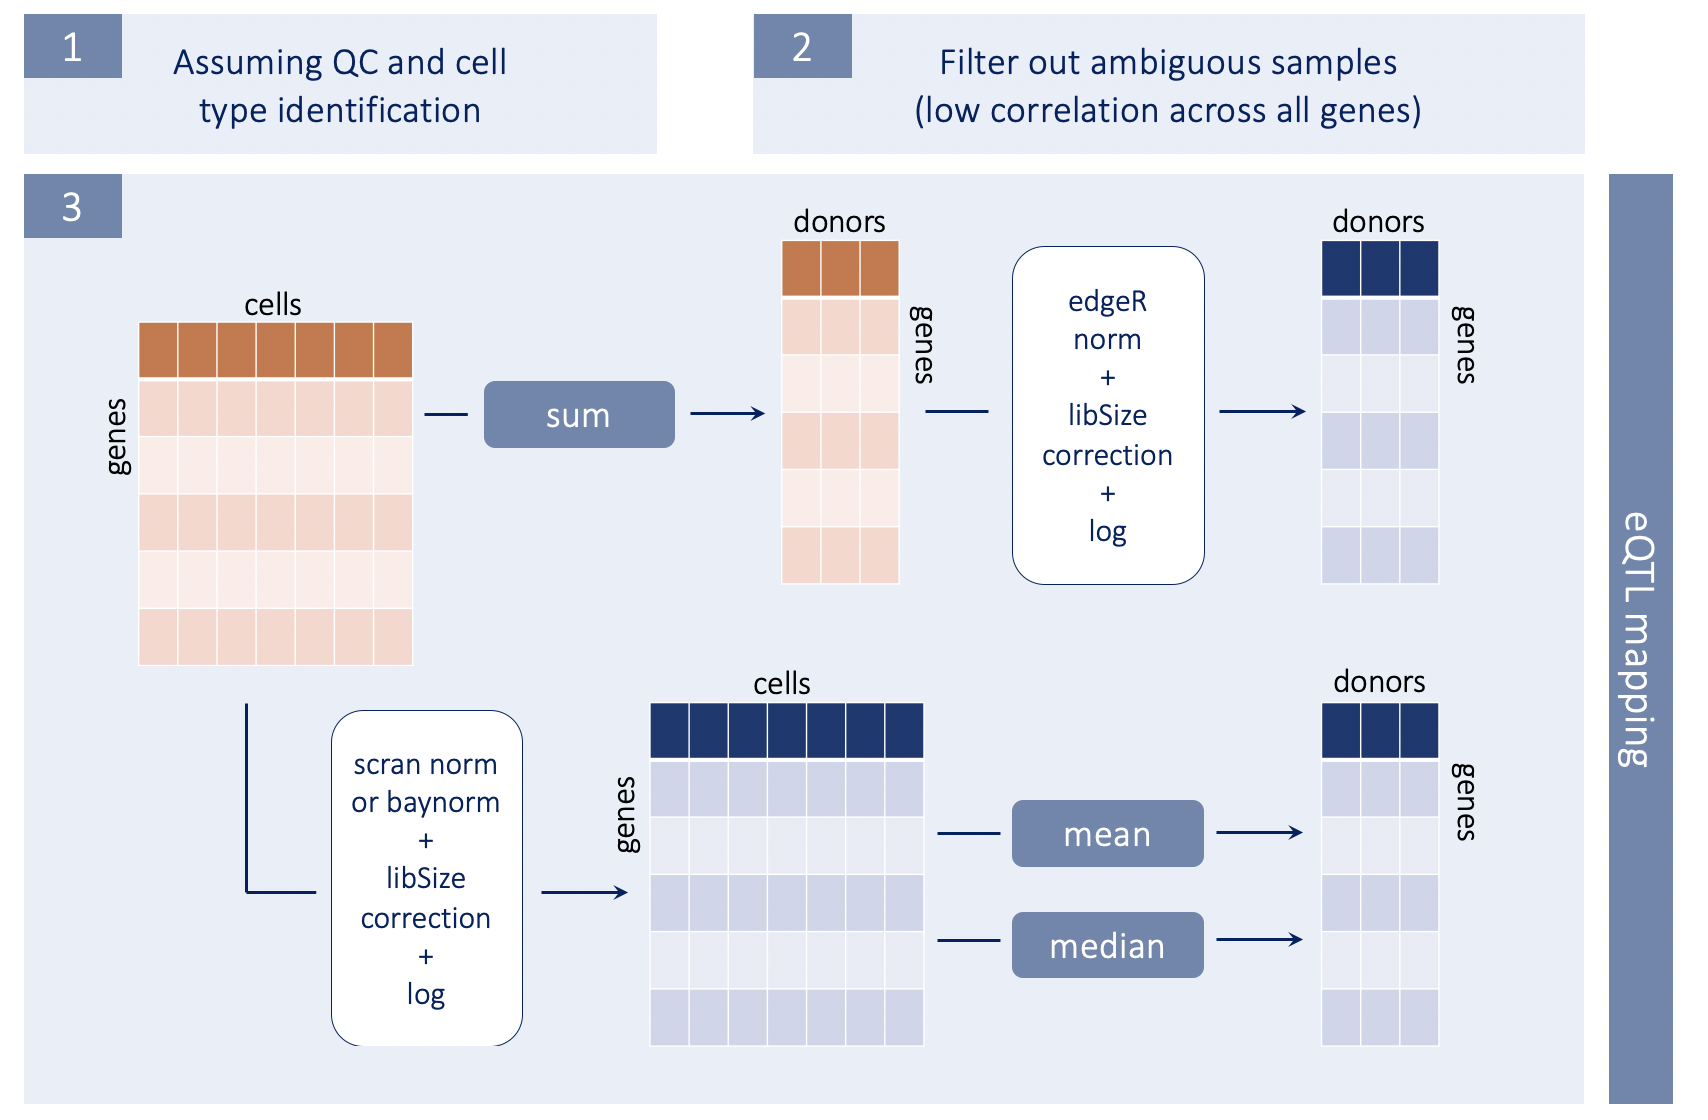
\includegraphics[width=15cm]{Chapter3/Fig/sc_qtl_workflow.png}
\caption[\textbf{sc-eQTL workflow}]{\textbf{sc-eQTL workflow}.\\
Placeholder: different approaches tested to perform eQTL mapping using scRNA-seq profiles}
\label{fig:sc_qtl_workflow}
\end{figure}

\begin{itemize}
    \item mean
    \item total mean
    \item median
    \item sum
    \item total sum
\end{itemize}

Aggregation is done at the donor level (i.e. all iPS cells from a given donor) in the mean, median and sum.
For what we call "total" sum and mean, on the other hand, aggregation (i.e. sum or mean) is done per donor and sequencing run, in an attempt to account for batch effects.

add details on normalization, 

\subsection{Covariates}

Another parameter we varied was the type and number of expression covariates included in the model to account for global expression variation (see section 2.X).

In particular, we computed principal components (PCs) from the (aggregated) expression matrix.
We also computed 10 MOFA factors \cite{argelaguet2018multi} as well as XX PEER factors \cite{stegle2010bayesian,stegle2012using}.

Since the total mean performed best as an aggregation method, we tested various number of covariates for this model only.

In particular, we included 5, 10, 20 and 50 PCs in the model as covariates and evaluated performance.

\section{Results in iPSCs}

\subsection{Comparison partners}

\begin{itemize}
    \item bulk RNA-seq with matched samples (i.e. individuals for which we have both bulk and sc-RNAseq data, N = 100)
    \item bulk RNA-seq all samples (i.e. all samples for which we have bulk RNA-seq data, N = 300)
    \item matched 10x scRNA-seq (for a subset of common samples, N = 30)
\end{itemize}


First, we tested for associations between common genetic variants and gene expression at iPSC stage. 
Briefly, for each donor, experimental batch, and differentiation stage, we quantified each gene’s average expression level, before using a linear mixed model to test for cis eQTL, adapting approaches described above and used for bulk RNA-seq profiles (+/- 250kb, MAF > 5\% \cite{kilpinen2017common}). 

\begin{equation}
    \boldsymbol{\mu} = \sum_i^{10}\alpha_i \mathbf{PC}_i + \mathbf{g}\beta + \mathbf{u} + \boldsymbol{\psi}  
\end{equation}

This identified 1,833 genes with at least one eQTL (denoted eGenes; FDR <10\%; 10,840 genes tested; Supplementary Data 3). 

% \section{Replication in bulk, 10x}

To validate our approach, we also performed eQTL mapping using deep bulk RNA-sequencing profiles from the same set of iPSC lines (“iPSC bulk”; 10,736 genes tested) generated as part of the HipSci project \cite{kilpinen2017common}, yielding consistent eQTL (~70\% replication of lead eQTL effects; nominal P<0.05; Methods; Supplementary Data 4).\\ 

These iPSC eQTL were further confirmed by analysis of scRNA-seq data generated from a subset of 5 experiments using a droplet-based approach (Methods; Supplementary Fig. 9, 10).


\section{Results in simulated data}





